\documentclass[12pt]{article}
\usepackage{../../template}
\title{Lecture 1}
\author{niceguy}
\begin{document}
\maketitle

\section{General Information}

No office hours scheduled; usually time left over after lectures.

\section{Introduction}

\subsection{The Basics of Fusion}

\begin{figure}
    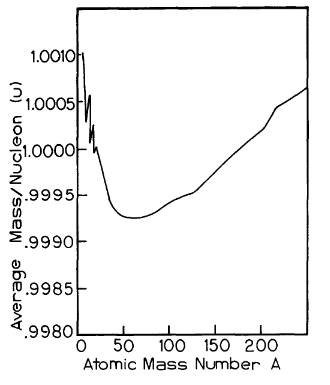
\includegraphics[width=0.5\textwidth]{1.png}
\end{figure}

Energy released is

\begin{equation}
    F = \Delta mc^2
\end{equation}

\subsection{Solar Reaction Chain}

\begin{align*}
    ^1\text{H} + ^1\text{H} &\rightarrow ^2\text{H} + e^+ + \gamma \\
    ^2\text{H} + ^1\text{H} &\rightarrow ^3\text{He} + \gamma \\
    ^3\text{He} + ^3\text{He} &\rightarrow ^4\text{He} + 2^1\text{H} + \gamma
\end{align*}

where the energies released are 0.41, 5.51, and 12.98 MeV respectively. The first step is rate determining, taking $\approx 7 \times 10^9$ years.

\subsection{Carbon Reaction Chain: heavier stars}

\begin{align*}
    ^{12}\text{C} + ^1\text{H} &\rightarrow ^{14}\text{N} + \gamma \\
    ^{13}\text{N} &\rightarrow ^{13}\text{C} + e^+ + \nu + \gamma \\
    ^{13}\text{C} + ^1\text{H} &\rightarrow ^{14}\text{N} + \gamma \\
    ^{14}\text{N} + ^1\text{H} &\rightarrow ^{15}\text{O} + \gamma \\
    ^{15}\text{O} &\rightarrow ^{15}\text{N} + e^+ + \nu + \gamma \\
    ^{15}\text{N} + ^1\text{H} &\rightarrow ^{12}\text{C} + ^4\text{He}
\end{align*}

Energies needed in MeV are 1.93, 1.20, 7.60, 7.39, 1.71, and 4.99 respectively.

\subsection{}

\begin{align*}
    \text{D} + \text{D} &\rightarrow \begin{cases} \text{T} (1.01) + p (3.03) & 50\% \\ ^3\text{He} (0.82) + n (2.45) & 50\% \end{cases} \\
    \text{D} + \text{T} &\rightarrow ^4\text{He} (3.52) + n (14.06) \\
    \text{D} + ^3\text{He} &\rightarrow ^4\text{He} (3.67) + p (14.67)
\end{align*}

Half lives of $n$ and T are 13 minutes and 12.4 years respectively.

\subsection{}

\begin{align*}
    ^6\text{Li} + \text{slow } n &\rightarrow \text{T} + ^4\text{He} \\
    ^7\text{Li} + \text{fast } n &\rightarrow \text{T} + ^4\text{He} + \text{slow } n
\end{align*}

Which take 4.8 and -2.5 MeV respectively.

\section{Contemporary Energy Consumption}

The ratio of sources of energy (fossil fuels, renewables, etc) has not changed since 2008, but we are using more and more fossil fuels, since energy demand is increasing. The optimistic view is that fossil fuels will run out before environment is "completely screwed up" (prof doesn't think so, since we're getting better at extracting them). Sustainable populations without fossil fuels or nuclear range from 0.5 - 2 billion, taking into account solar and wind power advances, plus conservation efforts. We have 50 - 100 years to find replacements for fossil fuels.

\begin{itemize}
    \item Nuclear fission \\
        Breeding plutonium from U238, or U233 from thorium, etc
    \item Solar power using space-based collectors \\
        Microwave power to Earth (how?)
    \item Fusion
\end{itemize}

\end{document}
